%%%%%%%%%%%%%%%%%%%%%%%%%%%%%%%%%%%%%%%%%%%%%%%%%%%%%%%%%%%%
% NGM Paper 2 — Case Studies (Overleaf / TRB)
% Companion to: NGM tool/framework paper (Paper 1)
%
% Overleaf setup:
%   1. Upload this folder (main.tex, references.bib)
%   2. Upload trbunofficial.cls (same class as Paper 1)
%   3. Upload composite PNGs under figs/ (see figs/README.md)
%   4. Compiler: pdfLaTeX (or XeLaTeX)
%%%%%%%%%%%%%%%%%%%%%%%%%%%%%%%%%%%%%%%%%%%%%%%%%%%%%%%%%%%%
\documentclass[numbered]{trbunofficial}

\hypersetup{colorlinks=true,urlcolor=black,linkcolor=black,citecolor=black}

% If booktabs is not loaded by the class, uncomment:
% \usepackage{booktabs}
\usepackage{amsmath}
\usepackage{multirow}
\usepackage{graphicx}
\usepackage{xcolor}

\begin{document}

\title{Operations and Safety Impacts of Connected and Automated Vehicles under
Imperfect V2X, Mixed Fleets, and Intersection Conflict Exposure:
Microsimulation Case Studies with NGM}

\TRBauthor{Pedram Beigi (Corresponding Author)}
{Department of Civil and Environmental Engineering, The George Washington University}
{beigi@gwu.edu}
[Washington, DC, USA, 20052]

\TRBauthor{Nachuan Li}
{Department of Civil and Environmental Engineering, Northwestern University}
{nachuan.li@northwestern.edu}
[Evanston, IL, USA, 60208]

\TRBauthor{Shayan Bafandkar}
{The Grainger College of Engineering, Department of Civil and Environmental Engineering,
University of Illinois at Urbana-Champaign}
{sbafan2@illinois.edu}
[Urbana, IL, USA, 61801]

\TRBauthor{John Hourdos, Ph.D.}
{Turner-Fairbank Highway Research Center, Federal Highway Administration}
{john.hourdos@dot.gov}
[McLean, VA, USA, 22101]

\TRBauthor{Yu (Marco) Nie, Ph.D.}
{Department of Civil and Environmental Engineering, Northwestern University}
{y-nie@northwestern.edu}
[Evanston, IL, USA, 60208]

\TRBauthor{Alireza Talebpour, Ph.D.}
{The Grainger College of Engineering, Department of Civil and Environmental Engineering,
University of Illinois at Urbana-Champaign}
{ataleb@illinois.edu}
[Urbana, IL, USA, 61801]

\TRBauthor{Samer H. Hamdar, Ph.D.}
{Department of Civil and Environmental Engineering, The George Washington University}
{hamdar@gwu.edu}
[Washington, DC, USA, 20052]

\AuthorHeaders{Beigi et al.}

\maketitle

% ============================================================
\section*{Abstract}
% ============================================================
Connected and automated vehicles (CAVs) are widely expected to improve freeway throughput,
dampen shockwaves, and reduce conflicts---yet these benefits depend on communication quality,
fleet mix, and facility type. Most planning-level CAV microsimulation studies still assume
ideal Vehicle-to-Everything (V2X) connectivity and investigate only passenger-car market
penetration, while safety assessments rarely compare cooperative CAVs against non-cooperative
automated vehicles (AVs) in the same VRU-rich intersection environment. This paper presents
four controlled microsimulation case studies executed with the open Next Generation Modeling
(NGM) platform, which couples trajectory-calibrated human models
(Prospect Theory car-following and Drift Diffusion lane changing) with cooperative C-IDM/C-MOBIL
controllers and a configurable V2X communication bus (range, latency, packet loss, and merge
intent). \emph{Case Study~1} isolates V2V reliability on a homogeneous CAV freeway and shows
that 50\% packet loss reduces mean speed by about 4\% versus ideal connectivity, whereas
1.0~s latency alone reduces speed by only about 1\%; the two stressors compound under combined
degradation. \emph{Case Study~2} demonstrates that CAV/CAHV penetration improves freeway and
especially arterial average speed and travel time relative to SV/HV baselines (arterial travel
time reductions of about 30\% at matched heavy-vehicle shares), that automating trucks helps
most when passenger traffic remains human-dominated, and that shockwave dynamics differ
systematically among SVs, AVs, and CAVs. \emph{Case Study~3} shows that at a signalized
intersection with pedestrians and bicycles, CAVs (and AVs) reduce critical rear-end
Time-to-Collision (TTC) events on links but do not clearly improve junction V2V conflicts and
can increase critical vehicle--pedestrian exposure. Across studies, results support a
planning guideline that imperfect V2X---particularly packet loss---should be treated as a
first-class scenario axis, and that CAV deployment benefits are facility- and mixed-fleet
dependent rather than uniformly positive. Replication scripts and baselines are released with
the NGM codebase.

\noindent\textbf{Keywords:} connected and automated vehicles; V2X reliability; market penetration;
surrogate safety; microsimulation; NGM

\newpage

% ============================================================
\section{Introduction}
\label{sec:intro}
% ============================================================
Agencies evaluating Connected and Automated Vehicle (CAV) strategies must answer questions that
go beyond idealized capacity adjustment factors: How much do latency and packet loss erode
cooperative platoon performance? How do mixed fleets of human-driven small vehicles (SVs),
heavy vehicles (HVs), CAVs, and connected automated heavy vehicles (CAHVs) reshape freeway weaving
and arterial throughput? Do cooperative controllers that improve rear-end safety on links also
reduce conflicts with pedestrians and cyclists at intersections? Answering these questions
requires controlled experiments in which behavioral models, communication quality, fleet mix,
and network geometry can be varied systematically while holding other factors constant.

A companion paper documents the open Next Generation Modeling (NGM) framework---an end-to-end
calibration-to-simulation tool linking trajectory-calibrated behavioral libraries to SUMO/TraCI
microsimulation with cooperative controllers and a V2X communication abstraction
\cite{BeigiNGMTool2026}. The present paper does \emph{not} rederive the tool architecture.
Instead, it reports a suite of operational and safety experiments designed to stress NGM's
distinctive capabilities: imperfect V2X, heterogeneous vehicle classes including heavy
vehicles, multi-facility scenarios (freeway weaves, arterials, and intersections with VRUs),
and surrogate safety metrics computed from high-resolution trajectories.

We organize the investigation into four case studies:

\begin{enumerate}
  \item \textbf{CS1 --- V2V reliability.} Homogeneous 100\% CAV freeway; sweep latency and
        packet loss relative to ideal connectivity and a human-driven baseline.
  \item \textbf{CS2 --- Market penetration and mixed fleets.} Freeway weaving and arterial OD
        demand under SV/HV versus CAV/CAHV compositions; complementary controlled shockwave
        experiments comparing SV, AV, and CAV streams.
  \item \textbf{CS3 --- Intersection safety.} Signalized single intersection with pedestrians
        and bicycles; 50/50 SV--CAV and SV--AV mixes; TTC criticality by interaction type and
        movement.
\end{enumerate}

The paper contributes empirical evidence on three under-addressed axes of CAV evaluation:
(i)~joint effects of latency and packet loss under cooperative control; (ii)~heavy-vehicle
automation (HV versus CAHV) interacting with passenger-car penetration; and (iii)~link versus
junction versus VRU safety patterns for cooperative and non-cooperative automation.
Section~\ref{sec:methods} summarizes the experimental platform and metrics.
Sections~\ref{sec:cs1}--\ref{sec:cs3} present the case studies. Section~\ref{sec:discuss}
synthesizes planning guidelines. Section~\ref{sec:conclusion} concludes.

% ============================================================
\section{Background and Related Work}
\label{sec:related}
% ============================================================
Microsimulation remains the primary tool for studying CAV operations before field deployment.
Commercial engines such as VISSIM, AIMSUN, and SUMO support mixed traffic, but often rely on
fixed car-following/lane-changing parameterizations or idealized information exchange
\cite{Krajzewski2012,ptvvissim2024}. Capacity-oriented CAV studies frequently report capacity
adjustment factors as a function of market penetration under Adaptive Cruise Control (ACC) or
Cooperative ACC (CACC) assumptions, typically with perfect or near-perfect connectivity and
passenger-car fleets \cite{Adebisi202X}. Such studies are invaluable for planning defaults but
leave open how imperfect V2X, trucks, and urban VRU interactions modify outcomes.

Communication-aware co-simulation frameworks (e.g., Veins, Plexe) couple traffic and network
simulators to study platooning under wireless imperfections \cite{segata2014plexe}. These
platforms emphasize protocol fidelity; behavioral extensibility and trajectory calibration are
often secondary. Conversely, empirical car-following/lane-changing literature based on
Prospect Theory, IDM, MOBIL, and Drift Diffusion Models improves behavioral realism
\cite{Treiber2000,Kesting2007,Talebpour2015,Ratcliff2008} but is rarely deployed in
full-corridor CAV scenario batteries with configurable latency/loss.

Surrogate safety assessments using Time-to-Collision (TTC), Post-Encroachment Time (PET), and
related measures are common for vehicle--vehicle and vehicle--VRU conflicts
\cite{Gettman2008SSAM,Lenard2018}. Comparative analyses of cooperative versus non-cooperative
automation at the same intersection---with identical demand, signals, and VRU presence---remain
less frequent.

This paper positions itself as an \emph{application} study built on NGM: calibrated human models
and cooperative CAV controllers are held fixed across scenarios so that differences can be
attributed to communication quality, fleet mix, or facility type rather than ad hoc retuning.

% ============================================================
\section{Experimental Platform and Metrics}
\label{sec:methods}
% ============================================================

\subsection{NGM simulation engines and vehicle classes}
All experiments use NGM Stage~2 runners with Eclipse SUMO and TraCI control \cite{BeigiNGMTool2026}.
Human-driven agents (SV, HV) and non-cooperative AVs sample longitudinal/lateral parameters
from trajectory-calibrated pools and operate with Prospect Theory (PT) car-following and Drift
Diffusion Model (DDM) lane changing in the registered case-study policy. Connected agents (CAV,
CAHV) use cooperative C-IDM longitudinal control and C-MOBIL lane changing informed by a
software \texttt{CommunicationBus} that applies communication range $R$, fixed-step latency
$\ell_{\mathrm{lat}}$, Bernoulli packet loss $p_{\mathrm{loss}}$, and virtual-vehicle merge
intent. Default lengths are 4.5~m for SV/AV/CAV and 12.0~m for HV/CAHV.

\subsection{V2X abstraction}
Each simulation step, connected vehicles broadcast
$(x,v,a,\ell,\mathrm{lane},\mathrm{tech})$. Ego vehicles query up to $M$ preceding connected
neighbors within range on the same lane. Lane-change intent is represented by a virtual vehicle
on the target lane with weight $\omega\in[0,1]$, allowing C-IDM to yield for merges. Unless noted
otherwise, CS1--CS2 connected scenarios use $R{=}30$~m and $M{=}3$ lookahead vehicles.

\subsection{Demand, duration, and replication}
Freeway and arterial simulations use a 0.1~s TraCI step. Freeway case studies run for
$T{=}1200$~s; arterial scenarios run for $T{=}1800$~s. Batch experiments are repeated with
seeded replicates; tables report means and standard deviations across runs unless otherwise
stated. Trajectory exporters produce per-vehicle time series for speed, travel time, EDIE-style
flow--density analysis, and TTC computation.

\subsection{Performance and safety metrics}
Operational metrics: \textbf{average speed} (m/s), \textbf{average travel time} (s), and
\textbf{flow--density} fundamental diagrams. Safety metrics in CS3: directional TTC for
same-lane rear-end pairs (V2V-1D), predictive 2-D TTC at intersection internals (V2V-2D), and
vehicle--pedestrian / vehicle--bicycle predictive TTC (V2Ped, V2Bike). A pair is labeled
\emph{critical} if its minimum TTC falls below the interaction-specific thresholds in
Table~\ref{tab:ttc_thresh} \cite{Lenard2018}.

\begin{table}[htbp]
  \centering
  \caption{Interaction-specific critical TTC thresholds used in Case Study~3.}
  \label{tab:ttc_thresh}
  \small
  \begin{tabular}{@{}lc@{}}
    \toprule
    Interaction & Critical TTC \\
    \midrule
    V2V & 1.5~s \\
    V2Ped & 1.2~s \\
    V2Bike & 1.8~s \\
    \bottomrule
  \end{tabular}
\end{table}

% ============================================================
\section{Case Study 1: Impact of V2V Reliability on Homogeneous CAV Freeway Flow}
\label{sec:cs1}
% ============================================================

\subsection{Design}
CS1 isolates communication quality under a \textbf{100\% CAV} fleet on a three-lane freeway
with a single on--off weave (geometry type \texttt{on\_off}). Ideal connectivity
($0$~s latency, $0\%$ packet loss) is compared against high latency ($1.0$~s), high packet
loss ($50\%$), mid combinations, and the joint worst case ($1.0$~s + $50\%$ loss). A
100\% SV human-driven baseline provides a non-connected reference. Demand (veh/h):
Main--Main $4500$, On--Main $300$, Main--Off $300$, On--Off $100$. Segment length is
1600~m with a 200~m ramp and a 300~m weave.

\begin{table}[htbp]
  \centering
  \caption{CS1 scenarios (communication sweep on 100\% CAV freeway; $R{=}30$~m, $M{=}3$).}
  \label{tab:cs1_scen}
  \small
  \begin{tabular}{@{}lll@{}}
    \toprule
    Scenario label & Latency & Packet loss \\
    \midrule
    100\% HDV (SV) baseline & --- & --- \\
    Ideal Connectivity & $0.0$~s & $0\%$ \\
    High Packet Loss & $0.0$~s & $50\%$ \\
    Mid Latency + Low Loss & $0.5$~s & $25\%$ \\
    Mid Latency + Mid Loss & $0.5$~s & $50\%$ \\
    High Latency & $1.0$~s & $0\%$ \\
    High Latency + High Loss & $1.0$~s & $50\%$ \\
    \bottomrule
  \end{tabular}
\end{table}

\subsection{Results}
Table~\ref{tab:cs1_results} summarizes mean speed and travel time. Ideal CAV connectivity
achieves $12.35$~m/s and $111.16$~s with very low run-to-run variability
($\sigma_{\mathrm{speed}}\approx 0.06$~m/s). Relative to ideal:

\begin{itemize}
  \item \textbf{Latency only ($1.0$~s):} speed $-1.1\%$ ($12.21$~m/s), travel time $+0.7\%$
        ($111.91$~s)---a mild systematic penalty; fundamental-diagram shape remains intact with
        mild peak-flow compression.
  \item \textbf{Packet loss only ($50\%$):} speed $-4.0\%$ ($11.85$~m/s), travel time $+1.7\%$
        ($113.06$~s); travel-time variability rises sharply
        ($\sigma\approx 3.83$~s versus $0.70$~s under ideal), indicating less stable
        platoon-level performance.
  \item \textbf{Combined stresses:} worst mean performance ($11.48$~m/s, $115.83$~s; about
        $-7.0\%$ speed and $+4.2\%$ travel time versus ideal). Impacts compound rather than
        add linearly: adding $50\%$ loss on top of $1.0$~s latency lowers speed by about
        $6\%$ versus the high-latency baseline, whereas adding $1.0$~s latency on top of
        $50\%$ loss lowers speed by about $3\%$ versus the high-loss baseline.
\end{itemize}

The homogeneous CAV ideal still outperforms the 100\% SV baseline ($11.31$~m/s, $121.92$~s),
confirming that cooperation recovers speed even before communication is stressed.
Corresponding mainline flow--density diagrams are shown in
Figures~\ref{fig:cs1_fd_base}--\ref{fig:cs1_fd_stress}.

\begin{table}[htbp]
  \centering
  \caption{CS1 average speed and travel time under V2V degradation (homogeneous CAV freeway
  unless noted).}
  \label{tab:cs1_results}
  \small
  \begin{tabular}{@{}lcccccc@{}}
    \toprule
    Scenario & Lat. & Loss & $\bar{v}$ (m/s) & $\overline{\mathrm{TT}}$ (s) & $\sigma_v$ & $\sigma_{\mathrm{TT}}$ \\
    \midrule
    100\% SV & --- & --- & 11.31 & 121.92 & 0.43 & 2.76 \\
    Ideal & 0.0~s & 0\% & 12.35 & 111.16 & 0.06 & 0.70 \\
    High Loss & 0.0~s & 50\% & 11.85 & 113.06 & 0.40 & 3.83 \\
    Mid Lat. + Low Loss & 0.5~s & 25\% & 12.11 & 112.07 & 0.27 & 1.88 \\
    Mid Lat. + Mid Loss & 0.5~s & 50\% & 11.81 & 113.14 & 0.26 & 1.69 \\
    High Latency & 1.0~s & 0\% & 12.21 & 111.91 & 0.24 & 1.64 \\
    High Lat. + High Loss & 1.0~s & 50\% & 11.48 & 115.83 & 0.45 & 4.51 \\
    \bottomrule
  \end{tabular}
\end{table}

\begin{figure}[htbp]
  \centering
  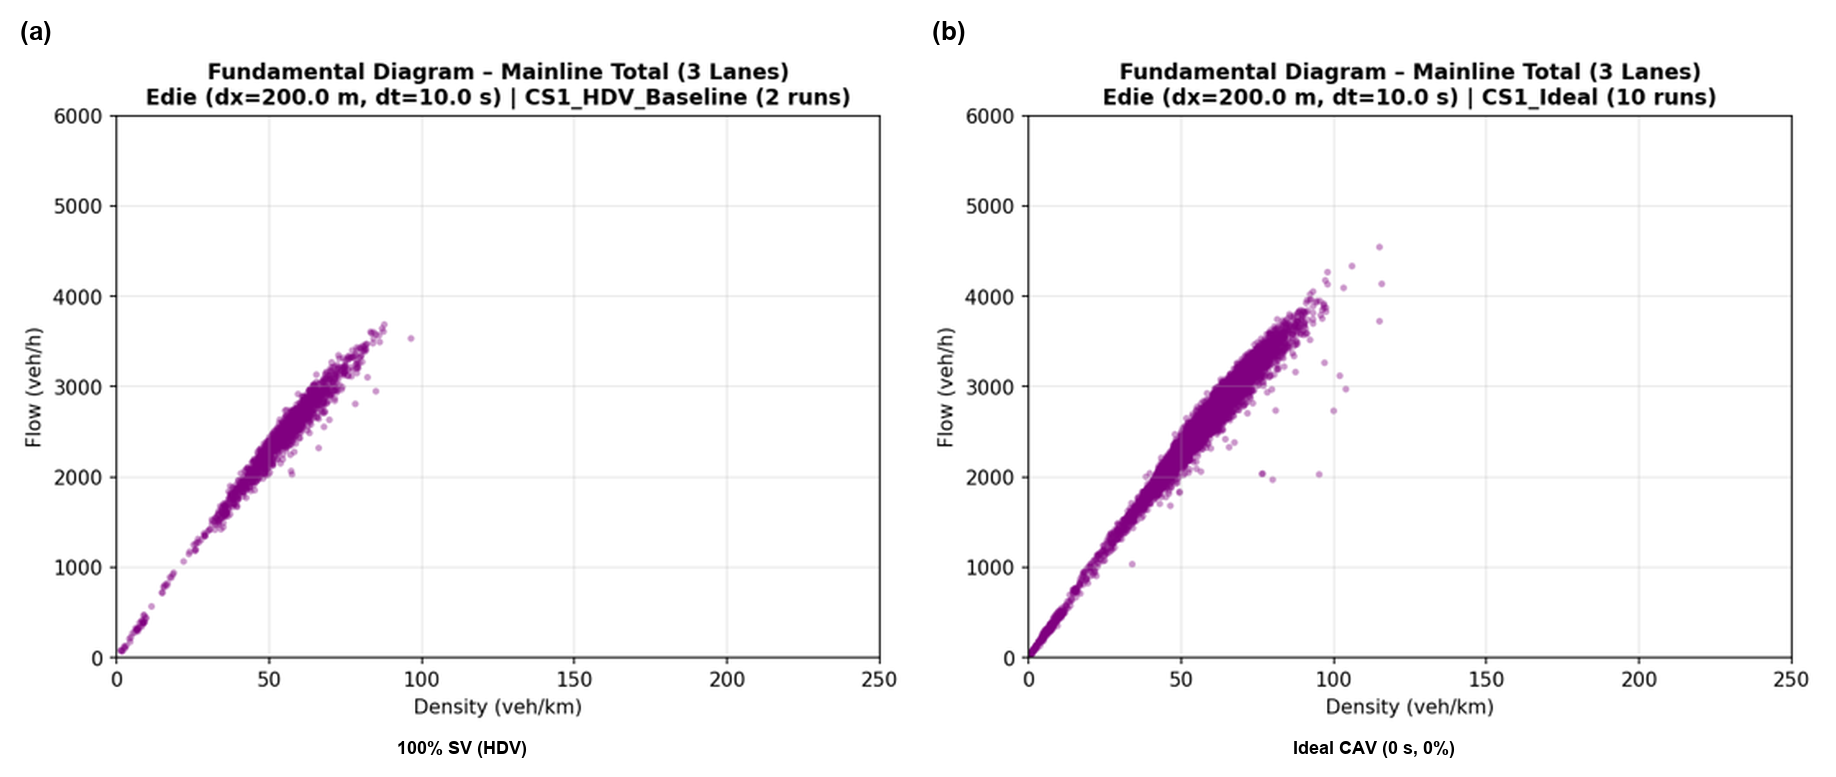
\includegraphics[width=\linewidth]{figs/fig_cs1_fd_baseline.png}
  \caption{Case Study~1 mainline flow--density diagrams: (a)~100\% SV (HDV) baseline;
  (b)~ideal CAV connectivity (0~s latency, 0\% loss).}
  \label{fig:cs1_fd_base}
\end{figure}

\begin{figure}[htbp]
  \centering
  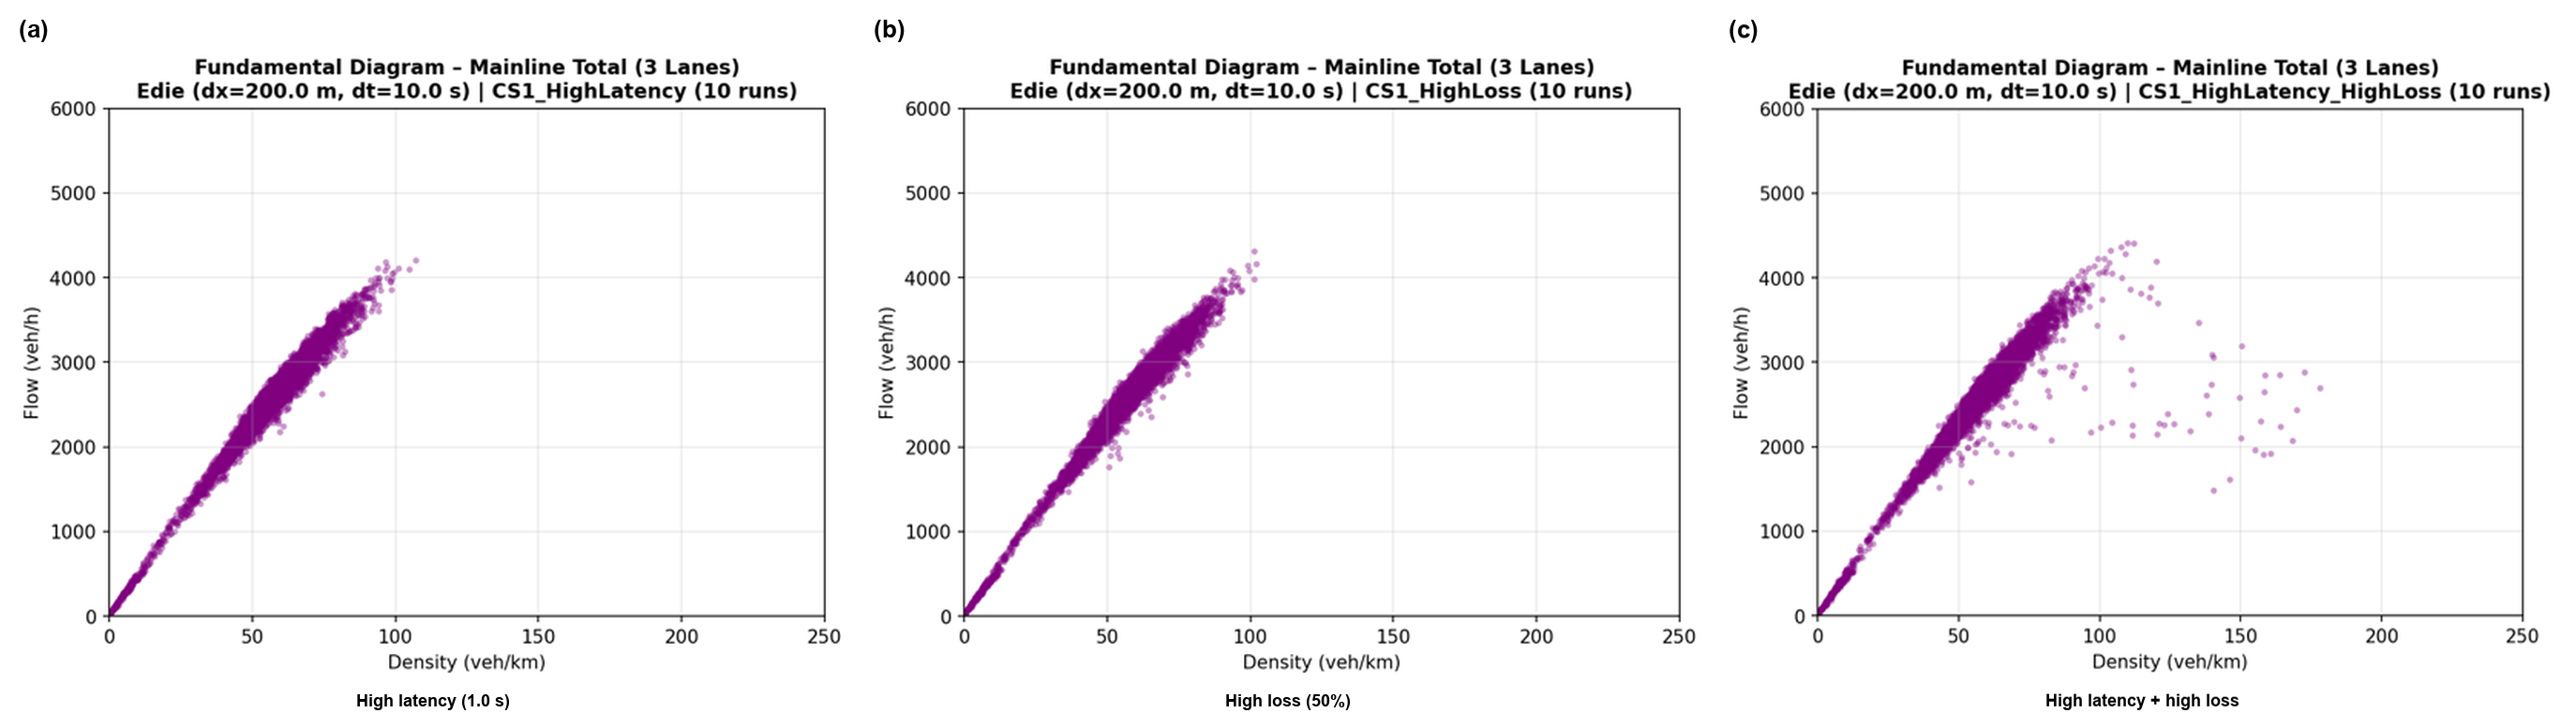
\includegraphics[width=\linewidth]{figs/fig_cs1_fd_stress.png}
  \caption{Case Study~1 mainline flow--density under V2V stress: (a)~high latency (1.0~s);
  (b)~high packet loss (50\%); (c)~combined high latency and high loss.
  Combined stress scatters the congested regime most strongly.}
  \label{fig:cs1_fd_stress}
\end{figure}

\subsection{Findings (CS1)}
Treating $1.0$~s latency and $50\%$ packet loss as equally ``extreme'' degradations,
\textbf{packet loss dominated mean performance impacts} in this non-congested homogeneous CAV
setting, while the \textbf{combination produced the worst outcomes}. Planning studies that
assume ideal V2X will overstate cooperative benefits; at minimum, separate sensitivity axes for
loss and latency are warranted, with joint stress cases included in robustness checks.

% ============================================================
\section{Case Study 2: Market Penetration, Mixed Fleets, and Shockwaves}
\label{sec:cs2}
% ============================================================

\subsection{Design}
CS2 evaluates operations under heterogeneous fleets on (i)~a dual-weave freeway
(\texttt{on\_off\_on\_off}, 1800~m, demand Main--Main $4500$~veh/h with ramp exchanges of
$300$/$100$~veh/h as specified in the experimental plan) and (ii)~a three-intersection arterial
with an OD matrix spanning through and turning movements (West--East through demand
$500$~veh/h each direction; remaining cells as reported in the companion technical report).
Fleet mixes include pure SV, SV/HV human baselines, balanced mixed traffic, and CAV/CAHV-dominant
compositions (Table~\ref{tab:cs2_results}). A parallel \textbf{shockwave} experiment forces
stops at $t{=}200$~s and $t{=}700$~s for $250$~s each on a controlled freeway stream of
homogeneous SVs, AVs, or CAVs to visualize propagation and dissipation.

\subsection{Freeway penetration results}
Table~\ref{tab:cs2_results} shows that the most degraded human freeway mix
(80\% SV / 20\% HV) yields the lowest mean speed among freeway runs ($10.21$~m/s). Full CAV
penetration achieves the best freeway operation ($12.11$~m/s, $117.63$~s). Matched-share
comparisons quantify the automation benefit:

\begin{itemize}
  \item $100\%$ CAV vs.\ $100\%$ SV: $+2.1\%$ speed, $-1.7\%$ travel time.
  \item $90\%$ CAV/$10\%$ CAHV vs.\ $90\%$ SV/$10\%$ HV: $+9.4\%$ speed, $-11.7\%$ travel time
        --- the largest travel-time reduction among equal-share comparisons.
  \item $80\%$ CAV/$20\%$ CAHV vs.\ $80\%$ SV/$20\%$ HV: $+7.9\%$ speed, $-5.5\%$ travel time.
\end{itemize}

A balanced mix (45\% CAV / 5\% CAHV / 45\% SV / 5\% HV) sits between pure SV and pure CAV
performance ($\bar{v}{=}11.63$~m/s) and clearly outperforms the congested human 90/10 and 80/20
HV mixes, confirming that even partial CAV penetration recovers operations under freight
stress.

Flow--density diagrams for matched freeway fleets show CAV-dominant curves extending toward
higher throughput and delaying breakdown relative to SV/HV baselines
(Figures~\ref{fig:cs2_fd_fwy_sv}--\ref{fig:cs2_fd_fwy_cav}).

\begin{figure}[htbp]
  \centering
  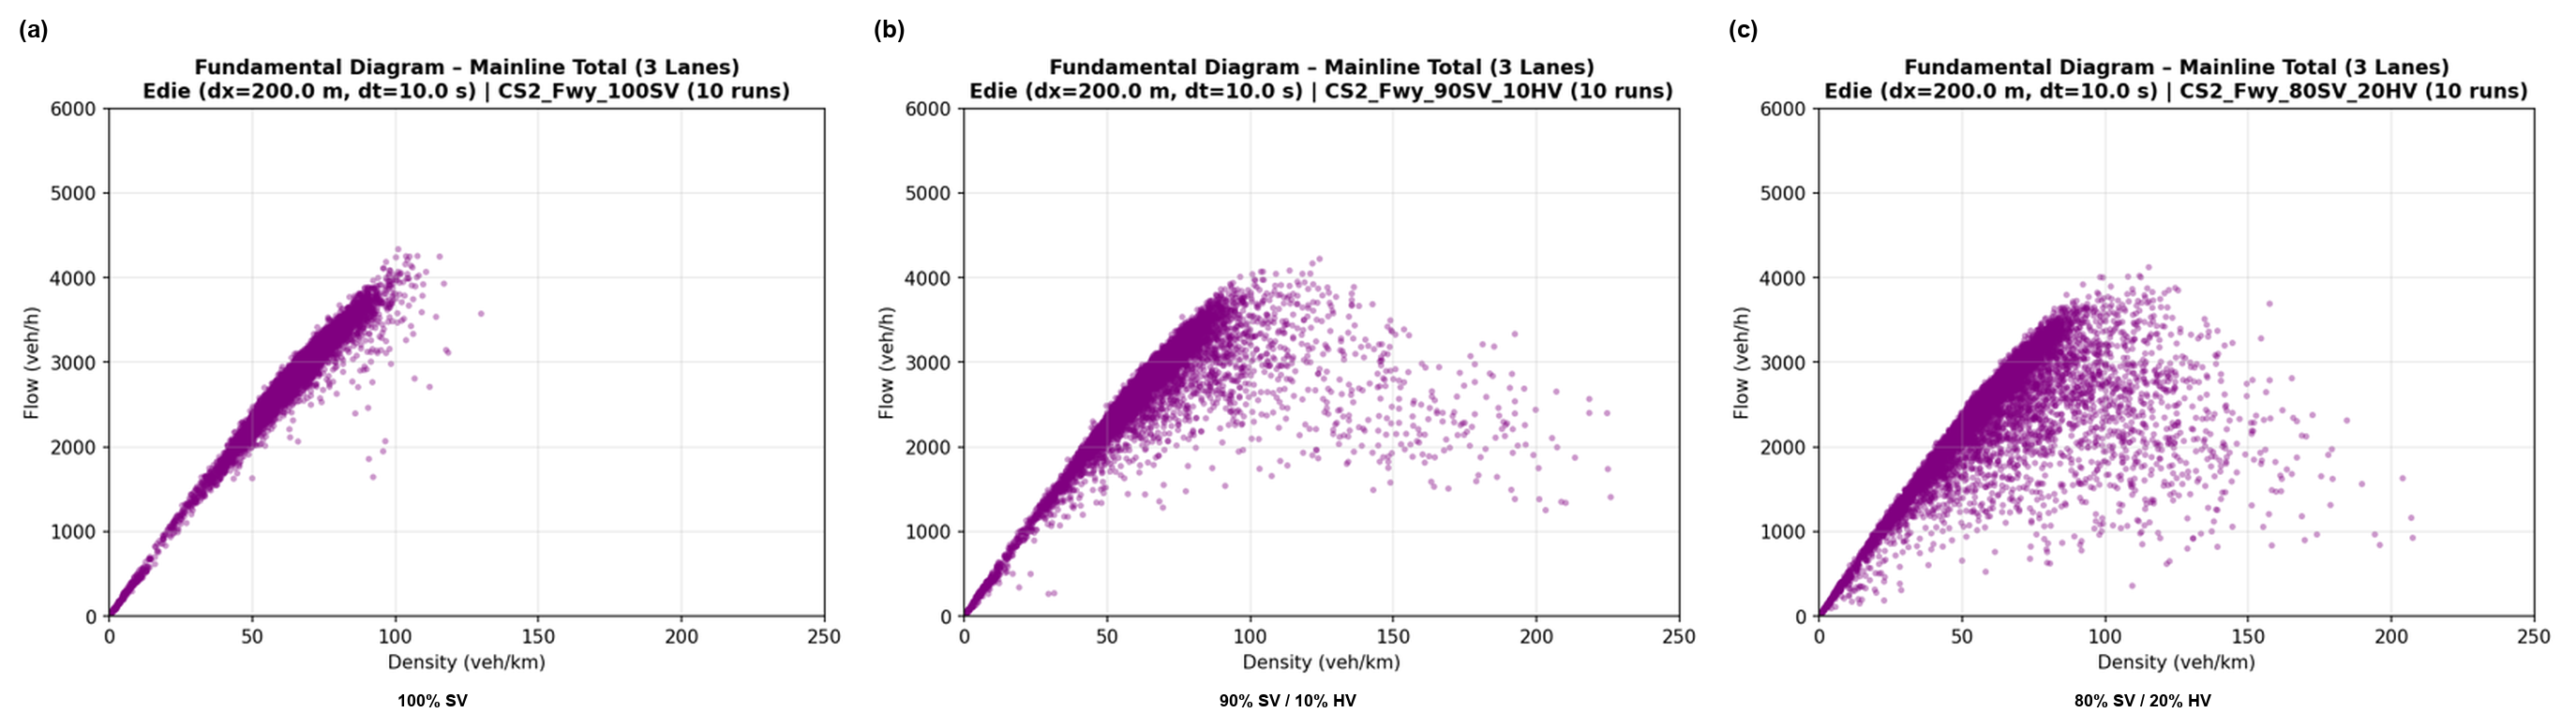
\includegraphics[width=\linewidth]{figs/fig_cs2_fd_freeway_sv.png}
  \caption{Case Study~2 freeway flow--density diagrams for human mixes:
  (a)~100\% SV; (b)~90\% SV / 10\% HV; (c)~80\% SV / 20\% HV.}
  \label{fig:cs2_fd_fwy_sv}
\end{figure}

\begin{figure}[htbp]
  \centering
  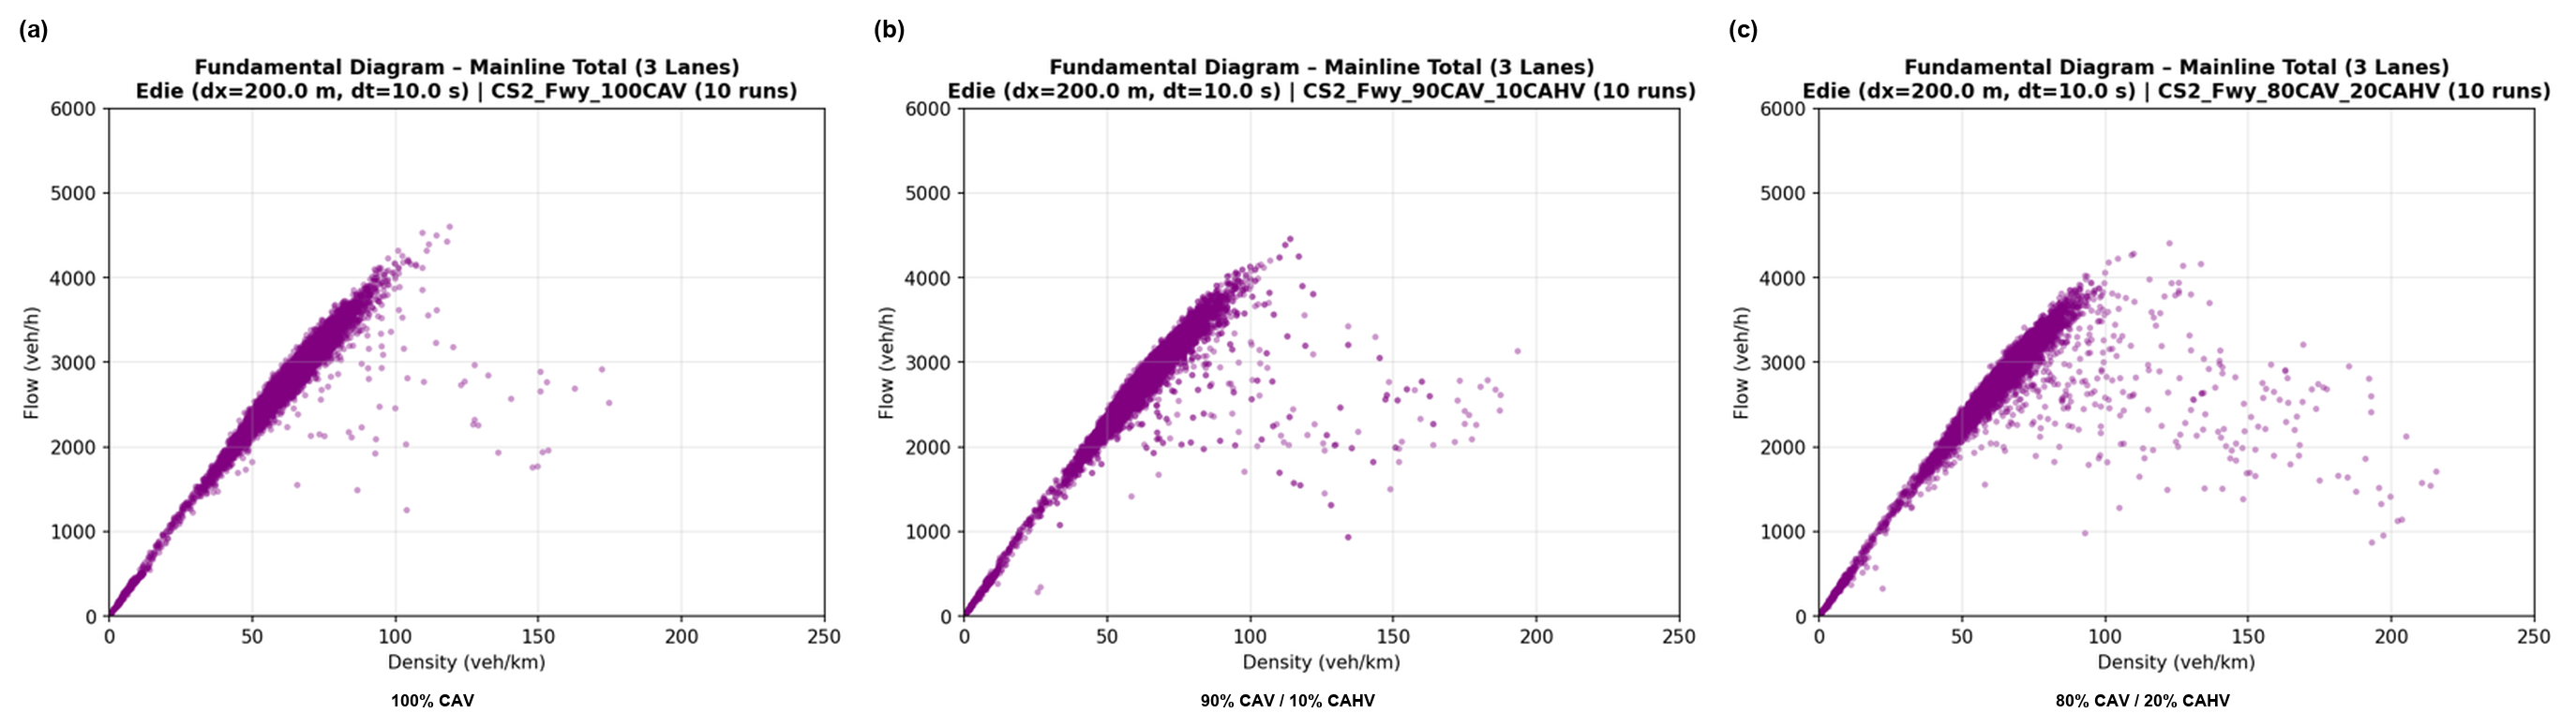
\includegraphics[width=\linewidth]{figs/fig_cs2_fd_freeway_cav.png}
  \caption{Case Study~2 freeway flow--density diagrams for connected mixes:
  (a)~100\% CAV; (b)~90\% CAV / 10\% CAHV; (c)~80\% CAV / 20\% CAHV.
  Relative to Figure~\ref{fig:cs2_fd_fwy_sv}, connected mixes extend toward higher
  throughput under freight stress.}
  \label{fig:cs2_fd_fwy_cav}
\end{figure}

\subsection{Arterial penetration results}
Arterial impacts are larger. Human mixes operate at roughly $4$--$5$~m/s with travel times of
$211$--$227$~s, whereas $90\%$ CAV/$10\%$ CAHV reaches $8.59$~m/s and $147.81$~s
(approximately $+69\%$ speed and $-30\%$ travel time versus $90\%$ SV/$10\%$ HV). The
$80\%$ CAV/$20\%$ CAHV mix similarly improves speed by about $+67\%$ and travel time by about
$-30\%$ versus its human twin. Fundamental diagrams on the arterial are reshaped toward higher
maximum flows under connected mixes, consistent with tighter spacing and cooperative gap
acceptance between signals (Figure~\ref{fig:cs2_fd_art}).

\begin{figure}[htbp]
  \centering
  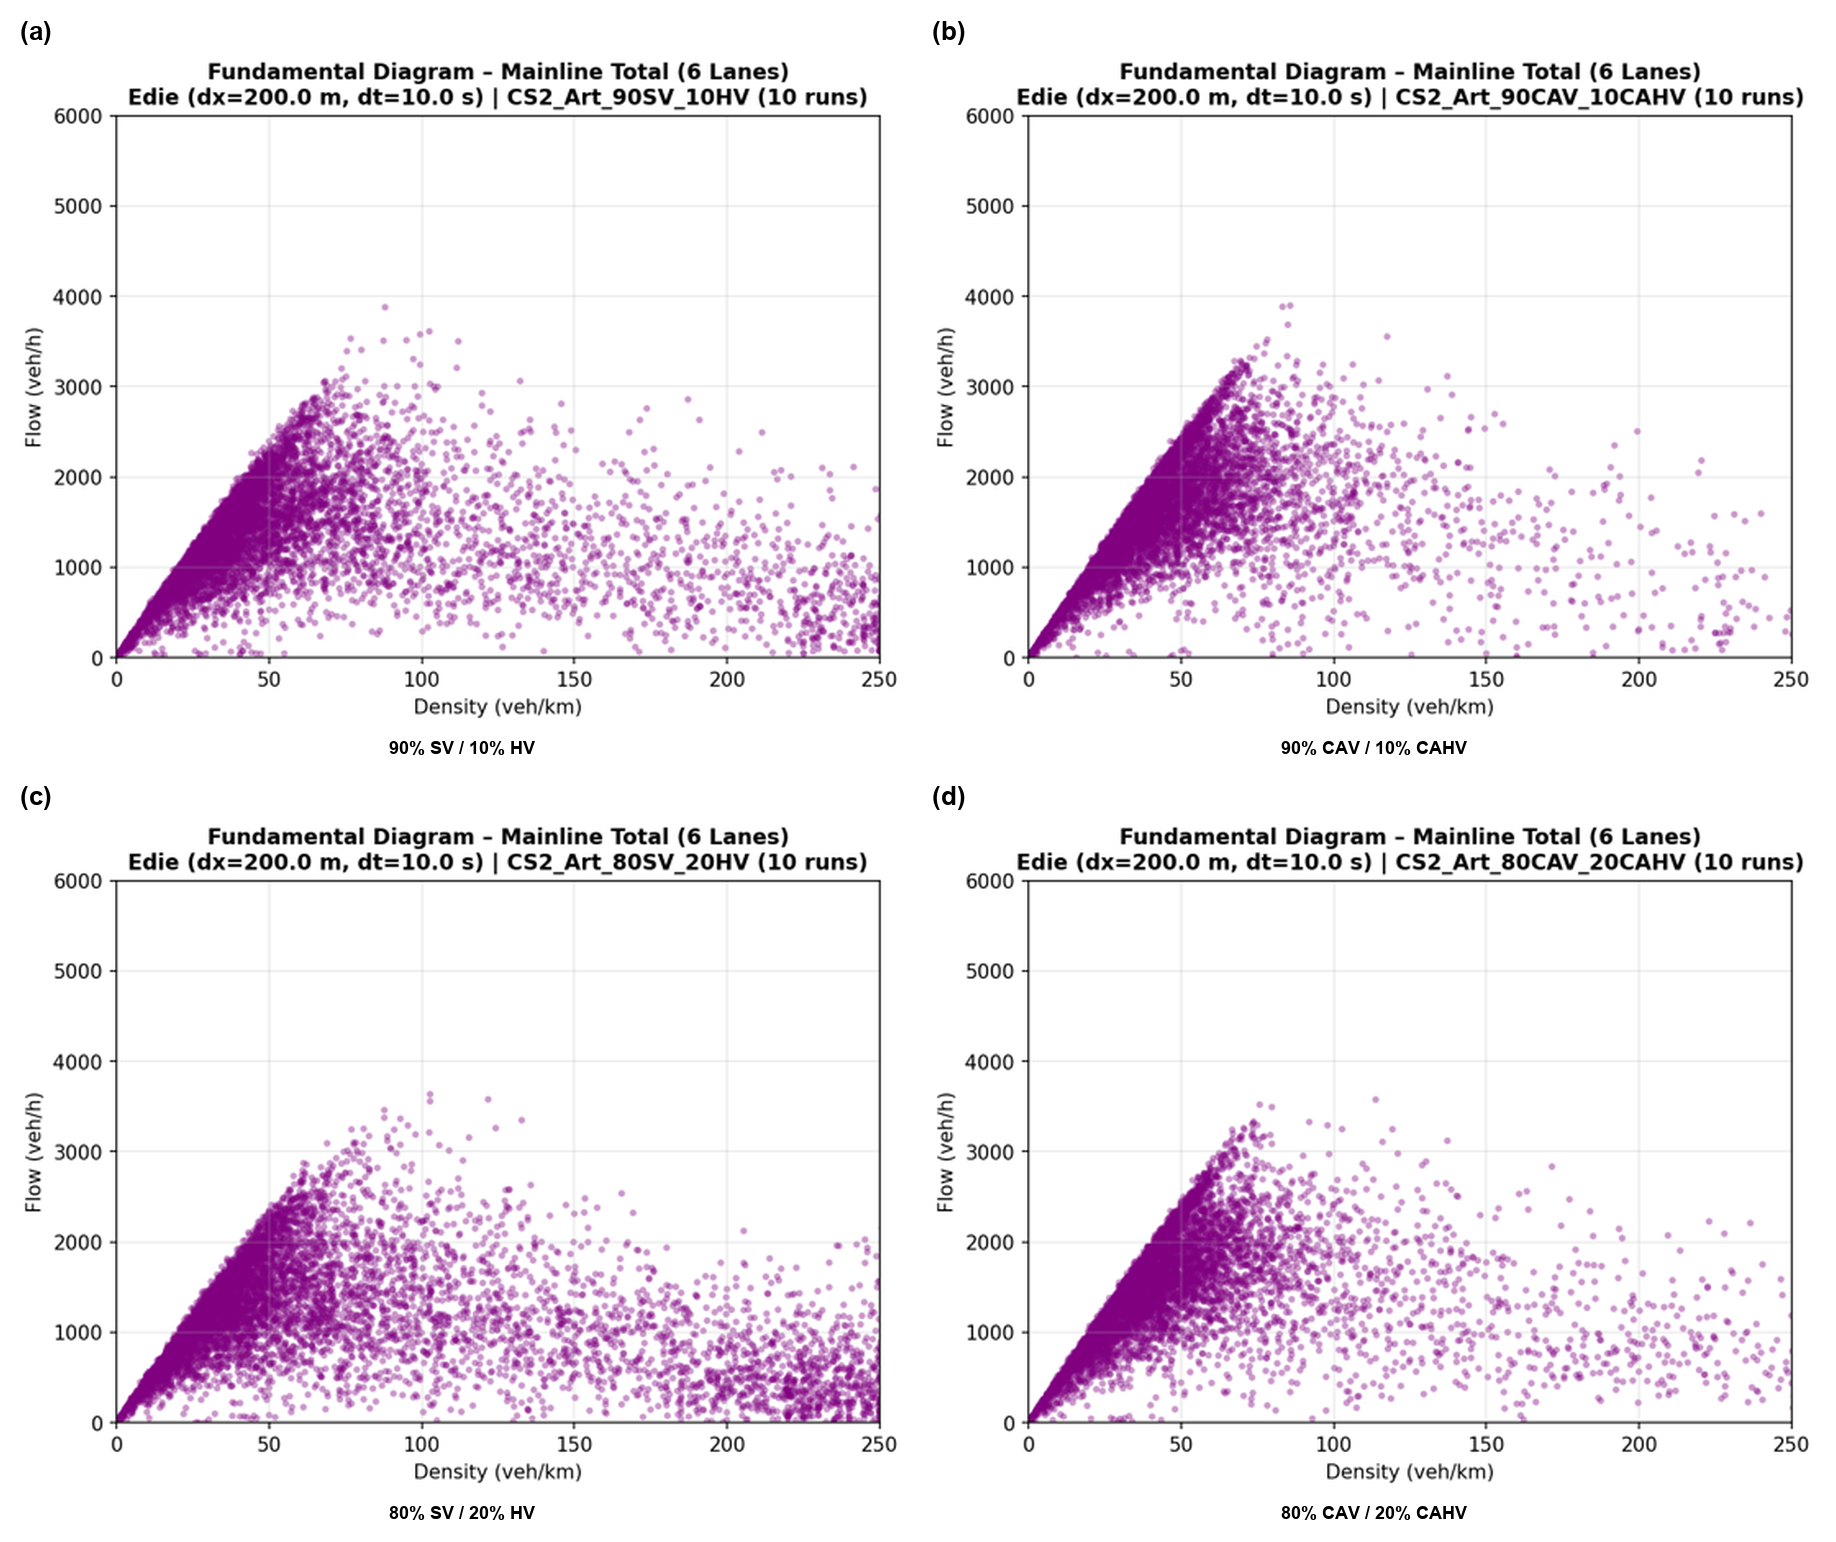
\includegraphics[width=\linewidth]{figs/fig_cs2_fd_arterial.png}
  \caption{Case Study~2 arterial flow--density diagrams: (a)--(b)~90\% SV/10\% HV vs.\
  90\% CAV/10\% CAHV; (c)--(d)~80\% SV/20\% HV vs.\ 80\% CAV/20\% CAHV.
  Connected mixes approximately double peak throughput relative to human baselines
  under the tested OD demand.}
  \label{fig:cs2_fd_art}
\end{figure}

\begin{table}[htbp]
  \centering
  \caption{CS2 average speed and travel time by environment and fleet mix.}
  \label{tab:cs2_results}
  \small
  \begin{tabular}{@{}llcccc@{}}
    \toprule
    Env. & Fleet mix & $\bar{v}$ & $\overline{\mathrm{TT}}$ & $\sigma_v$ & $\sigma_{\mathrm{TT}}$ \\
    \midrule
    Freeway & 100\% SV & 11.86 & 119.65 & 0.28 & 2.53 \\
    Freeway & 90\% SV / 10\% HV & 10.85 & 136.04 & 1.01 & 12.54 \\
    Freeway & 80\% SV / 20\% HV & 10.21 & 135.87 & 2.03 & 32.47 \\
    Freeway & 45\% CAV/5\% CAHV / 45\% SV/5\% HV & 11.63 & 122.95 & 0.94 & 11.14 \\
    Freeway & 100\% CAV & 12.11 & 117.63 & 0.22 & 2.23 \\
    Freeway & 90\% CAV / 10\% CAHV & 11.87 & 120.18 & 0.64 & 7.01 \\
    Freeway & 80\% CAV / 20\% CAHV & 11.02 & 128.42 & 0.92 & 12.04 \\
    Freeway & 90\% SV / 10\% CAHV & 11.57 & 121.65 & 0.39 & 2.63 \\
    Freeway & 90\% CAV / 10\% HV & 11.78 & 120.92 & 0.77 & 8.51 \\
    Arterial & 90\% SV / 10\% HV & 5.08 & 210.78 & 1.27 & 34.65 \\
    Arterial & 80\% SV / 20\% HV & 4.37 & 227.02 & 0.75 & 25.64 \\
    Arterial & 90\% CAV / 10\% CAHV & 8.59 & 147.81 & 1.66 & 28.52 \\
    Arterial & 80\% CAV / 20\% CAHV & 7.29 & 159.94 & 1.41 & 19.84 \\
    \bottomrule
  \end{tabular}
\end{table}

\subsection{Heavy-vehicle automation: HV versus CAHV}
Cross-comparisons at a fixed 90/10 majority/minority split clarify where truck automation pays
off. Replacing the 10\% HV share with CAHV inside an SV-dominated stream raises speed by about
$6.6\%$ and cuts travel time by about $10.6\%$ ($10.85\rightarrow 11.57$~m/s). Automating the
passenger majority (SV$\rightarrow$CAV) while keeping 10\% HV yields still larger improvements
($+8.6\%$ speed). Once passenger traffic is already highly connected (90\% CAV), switching the
10\% truck share from HV to CAHV changes macroscopic averages only marginally ($+0.8\%$ speed).
Thus, \textbf{passenger-car connectivity absorbs freight disruption}; truck automation delivers
its largest network-level returns while surrounding traffic remains mostly human-driven.
Figure~\ref{fig:cs2_fd_truck} shows the corresponding freeway fundamental diagrams for the
90\% SV/10\% CAHV and 90\% CAV/10\% HV cross-mixes.

\begin{figure}[htbp]
  \centering
  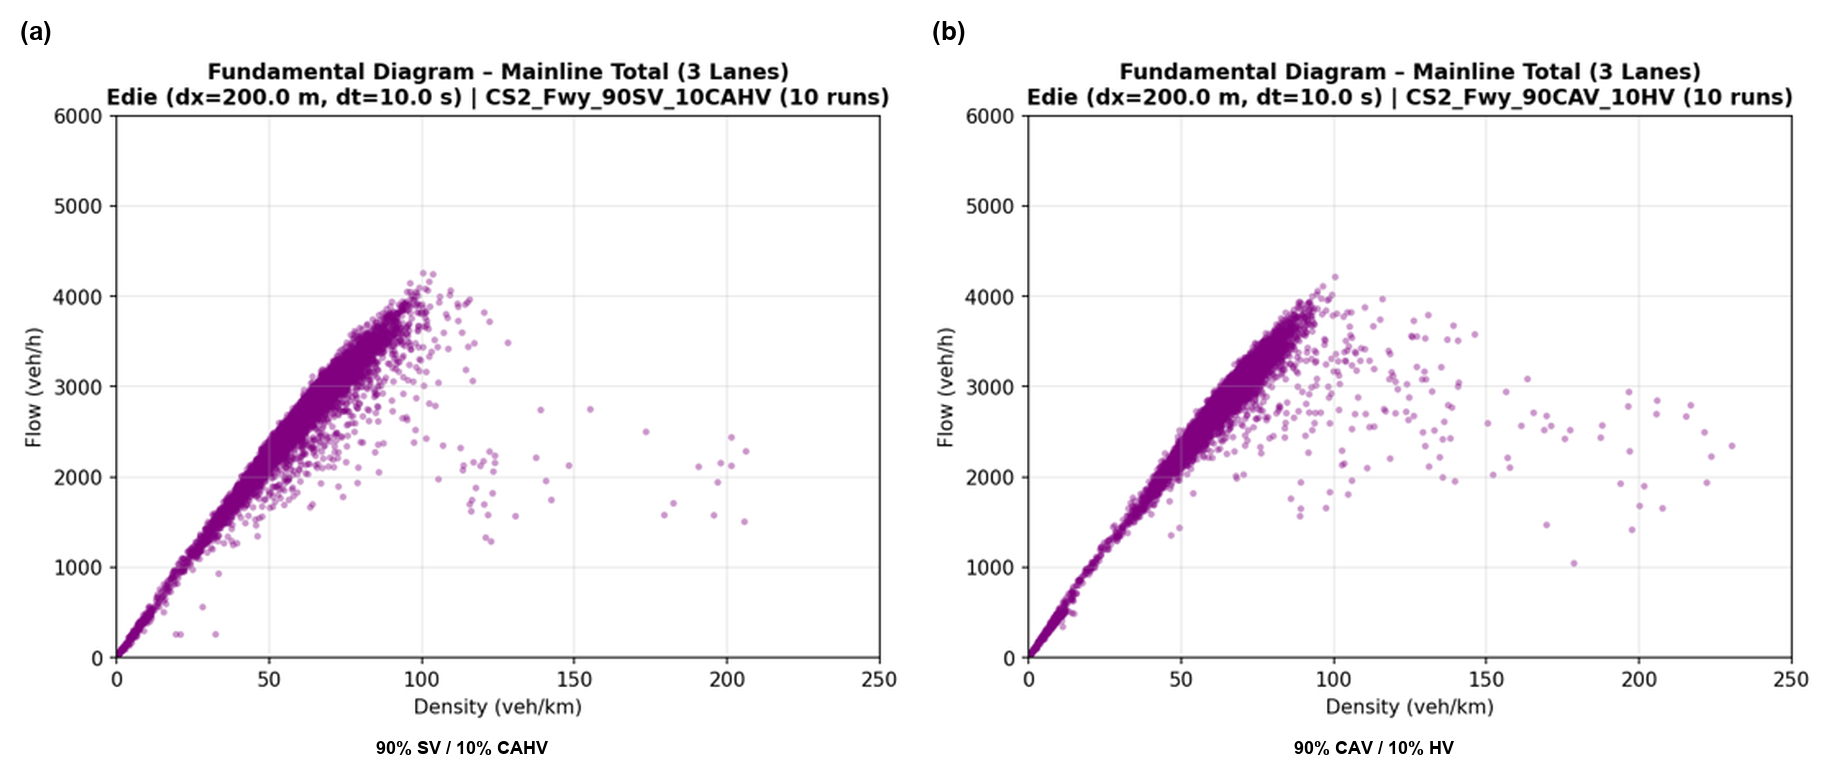
\includegraphics[width=0.95\linewidth]{figs/fig_cs2_fd_truck.png}
  \caption{Case Study~2 freeway flow--density for heavy-vehicle cross-mixes at a fixed
  90/10 split: (a)~90\% SV / 10\% CAHV; (b)~90\% CAV / 10\% HV.}
  \label{fig:cs2_fd_truck}
\end{figure}

\subsection{Shockwave propagation (SV vs.\ AV vs.\ CAV)}
Controlled stop-and-go experiments reveal qualitative differences in space--time diagrams.
Non-cooperative AVs synchronize identical car-following responses and sustain strong
backward-propagating waves. CAVs, using V2V lookahead, anticipate stops and smooth
deceleration, mitigating wave amplitude relative to AVs. Heterogeneous SVs often clear
disruptions more effectively than rigid AV platoons because behavioral variability acts as an
organic damper. These results caution against equating ``automation'' with ``cooperation'':
without V2X, homogeneous AVs can worsen string stability relative to mixed human traffic under
the tested disruption protocol. CAV dissipation remains communication-parameter dependent
(range, lookahead). Figure~\ref{fig:cs2_shockwave} compares space--time diagrams across
SV, AV, and CAV streams.

\begin{figure}[htbp]
  \centering
  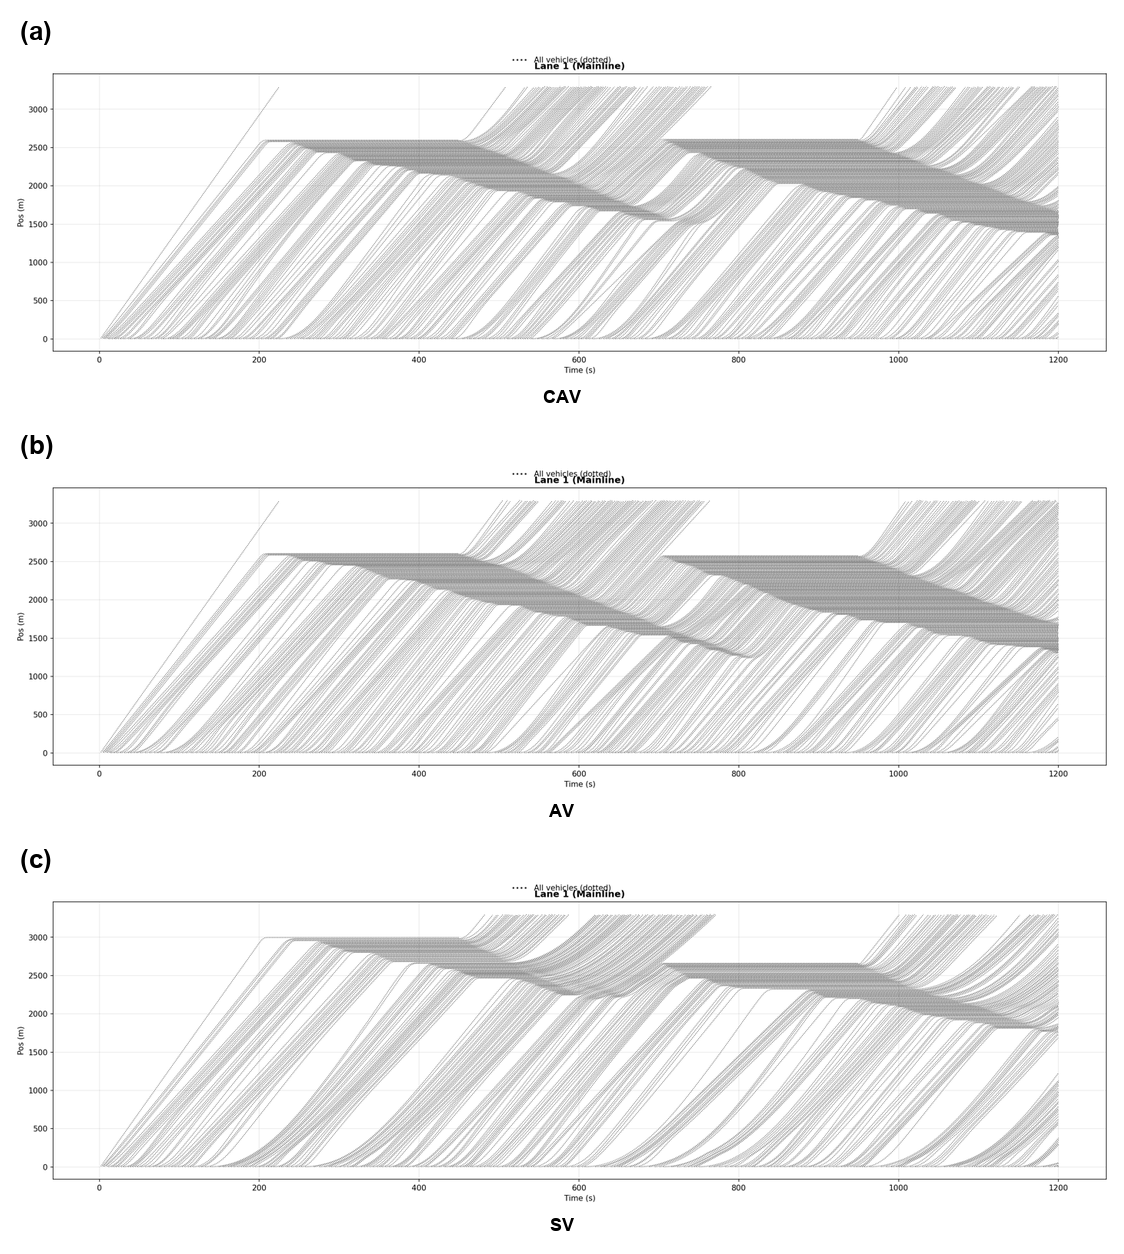
\includegraphics[width=0.92\linewidth]{figs/fig_cs2_shockwave.png}
  \caption{Controlled shockwave propagation and dissipation for homogeneous (a)~CAV,
  (b)~AV, and (c)~SV streams under forced stops at $t{=}200$~s and $t{=}700$~s
  (panels stacked top to bottom). Non-cooperative AVs sustain strong backward waves;
  CAVs damp disruptions via V2V lookahead; heterogeneous SVs can clear waves via
  behavioral variability.}
  \label{fig:cs2_shockwave}
\end{figure}

\subsection{Findings (CS2)}
CAV/CAHV penetration improves mean operations on freeways and, more strongly, on arterials.
Benefits scale with heavy-vehicle friction in human baselines. Truck automation should be
prioritized earlier when passenger fleets are still largely human; once CAV passenger
penetration is high, remaining HV/CAHV mix has second-order macroscopic effects. Shockwave
behavior highlights that connectivity---not automation alone---is the key mechanism for
cooperative damping in these experiments.

% ============================================================
\section{Case Study 3: Intersection Safety with Mixed Automation and VRUs}
\label{sec:cs3}
% ============================================================

\subsection{Design}
CS3 uses a signalized single-intersection environment with pedestrians and bicycles enabled.
Two 50/50 vehicle mixes are compared: \textbf{SV--CAV} and \textbf{SV--AV}. Trajectories are
segmented by agent group. Safety is quantified by critical TTC rates and median TTC for
V2V-1D (link rear-end), V2V-2D (intersection), V2Ped, and V2Bike interactions
(Table~\ref{tab:ttc_thresh}).

\subsection{SV versus CAV results}
Table~\ref{tab:cs3_cav} summarizes surrogate safety by interaction type. On \textbf{V2V-1D}
links, CAVs reduce the critical rate from $10.5\%$ to $4.3\%$ (median TTC: $3.59$~s vs.\
$4.86$~s for humans---note that criticality focuses on the left tail below the threshold). At
the junction (\textbf{V2V-2D}), rates are effectively unchanged ($5.1\%$ vs.\ $5.3\%$). For
\textbf{VRUs}, critical rates \emph{increase} for CAVs: V2Ped $27.0\%\rightarrow 32.4\%$;
V2Bike $46.5\%\rightarrow 50.3\%$.

Movement-level analysis shows the strongest CAV rear-end gains on left-turn link conflicts
($19.5\%\rightarrow 4.3\%$ critical) and left-turn bike interactions
($66.7\%\rightarrow 41.7\%$), while through movements---which carry most exposure---still
improve V2V-1D but worsen V2Ped ($25.1\%\rightarrow 32.8\%$) and V2Bike
($46.7\%\rightarrow 58.1\%$). Empirical CDFs of minimum TTC by interaction type are shown in
Figure~\ref{fig:cs3_ttc}.

\begin{figure}[htbp]
  \centering
  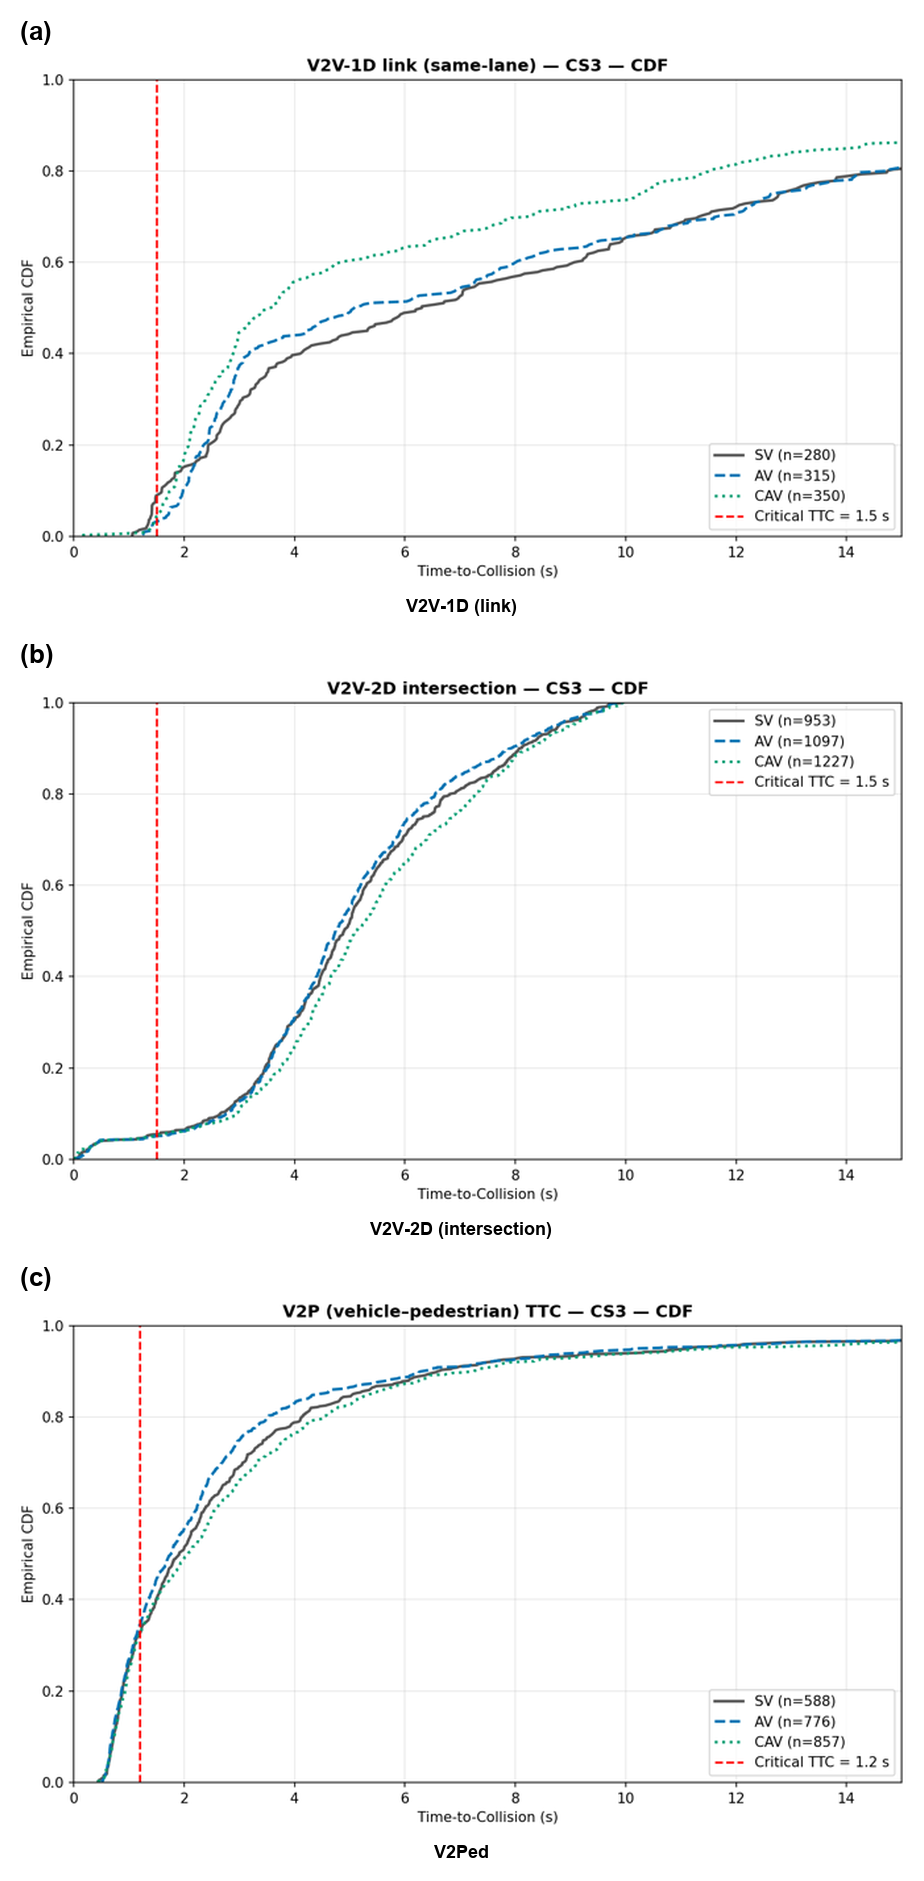
\includegraphics[width=0.72\linewidth]{figs/fig_cs3_ttc_cdf.png}
  \caption{Empirical CDFs of minimum TTC comparing SV, AV, and CAV groups:
  (a)~V2V-1D link rear-end; (b)~V2V-2D intersection; (c)~V2Ped.
  Vertical dashed lines mark critical thresholds in Table~\ref{tab:ttc_thresh}.}
  \label{fig:cs3_ttc}
\end{figure}

\begin{table}[htbp]
  \centering
  \caption{CS3 surrogate safety for 50/50 SV--CAV mix by interaction type.}
  \label{tab:cs3_cav}
  \small
  \begin{tabular}{@{}llcccc@{}}
    \toprule
    Interaction & Group & Pairs & TTC$_{\mathrm{med}}$ (s) & Critical & Rate \\
    \midrule
    V2V-1D & Human & 399 & 4.86 & 42 & 10.53\% \\
    V2V-1D & CAV & 350 & 3.59 & 15 & 4.29\% \\
    V2V-2D & Human & 1245 & 5.19 & 63 & 5.06\% \\
    V2V-2D & CAV & 1227 & 5.10 & 65 & 5.30\% \\
    V2Ped & Human & 773 & 2.06 & 209 & 27.04\% \\
    V2Ped & CAV & 857 & 2.07 & 278 & 32.44\% \\
    V2Bike & Human & 172 & 1.99 & 80 & 46.51\% \\
    V2Bike & CAV & 165 & 1.79 & 83 & 50.30\% \\
    \bottomrule
  \end{tabular}
\end{table}

\subsection{SV versus AV results}
In the non-cooperative 50/50 SV--AV mix (Table~\ref{tab:cs3_av}), V2V-1D criticality again falls
sharply for AVs ($8.9\%\rightarrow 3.2\%$), while V2V-2D remains nearly neutral
($5.5\%\rightarrow 5.1\%$). VRU patterns are mixed: V2Ped slightly worse for AVs
($32.7\%\rightarrow 34.5\%$); V2Bike modestly better ($48.7\%\rightarrow 45.0\%$). Thus,
\textbf{link rear-end safety gains appear with automation even without cooperation}, whereas
junction neutrality and uneven VRU outcomes persist---implying that cooperative gap/merge
logic alone does not automatically transfer safety benefits to crossing pedestrians and
cyclists under the tested Social Force / PT-VRU behaviors and perception assumptions.

\begin{table}[htbp]
  \centering
  \caption{CS3 surrogate safety for 50/50 SV--AV mix by interaction type.}
  \label{tab:cs3_av}
  \small
  \begin{tabular}{@{}llcccc@{}}
    \toprule
    Interaction & Group & Pairs & TTC$_{\mathrm{med}}$ (s) & Critical & Rate \\
    \midrule
    V2V-1D & SV & 280 & 6.31 & 25 & 8.93\% \\
    V2V-1D & AV & 315 & 5.09 & 10 & 3.18\% \\
    V2V-2D & SV & 953 & 4.90 & 52 & 5.46\% \\
    V2V-2D & AV & 1097 & 4.74 & 56 & 5.11\% \\
    V2Ped & SV & 588 & 1.91 & 192 & 32.65\% \\
    V2Ped & AV & 776 & 1.76 & 268 & 34.54\% \\
    V2Bike & SV & 113 & 1.86 & 55 & 48.67\% \\
    V2Bike & AV & 171 & 1.92 & 77 & 45.03\% \\
    \bottomrule
  \end{tabular}
\end{table}

\subsection{Findings (CS3)}
CAVs (and AVs) improve critical rear-end exposure on approach links---especially left-turn
related link conflicts for CAVs---but do not clearly improve intersection V2V conflicts and
may increase pedestrian/bicycle criticality under current controller assumptions. Deployment
narratives that equate CAV penetration with ``safer intersections'' need facility- and
VRU-specific evidence; link-level TTC improvements are not a sufficient proxy.

% ============================================================
\section{Cross-Cutting Discussion and Planning Guidelines}
\label{sec:discuss}
% ============================================================
Synthesizing CS1--CS3 yields the following guidelines for agencies and modelers:

\begin{enumerate}
  \item \textbf{Do not assume ideal V2X.} Packet loss can dominate latency for mean freeway
        speed under homogeneous CAV cooperation; joint latency$\times$loss cases produce the
        worst outcomes and should be included in robustness analysis.
  \item \textbf{Facility type matters.} Relative CAV benefits are larger on the congested
        arterial OD network than on the dual-weave freeway under the tested demands.
  \item \textbf{Treat trucks explicitly.} SV/HV mixes are the most fragile baselines;
        automating passenger cars in freight-heavy traffic yields large travel-time returns.
        CAHV investments matter most while passenger fleets remain human-dominated.
  \item \textbf{Automation $\neq$ cooperation for stability.} Controlled shockwaves show
        non-cooperative AVs can sustain stronger waves than heterogeneous humans; V2X-enabled
        CAVs damp disruptions more effectively.
  \item \textbf{Safety is interaction-specific.} Rear-end critical TTC can fall while
        VRU-critical rates rise. Intersection CAV evaluation must report V2V-2D and VRU
        metrics separately from link rear-end TTC.
\end{enumerate}

Limitations include fixed-step latency, Bernoulli loss (no burst/congestion RF models),
idealized intent via virtual vehicles, a single VRU corridor parameterization for
pedestrian/bicycle dynamics, and kinematic limits inherited from SUMO. Results should be
interpreted as controlled comparative evidence under NGM's behavioral/communication stack
rather than universal constants for all CAV stacks.

% ============================================================
\section{Conclusions}
\label{sec:conclusion}
% ============================================================
This paper reported four microsimulation case studies executed with the open NGM platform to
quantify CAV operations and safety under imperfect V2X, mixed SV/HV/CAV/CAHV fleets, and
intersection conflicts with VRUs. On a homogeneous CAV freeway, packet loss degraded mean
performance more than an equally ``extreme'' latency of $1.0$~s, and the stressors compounded.
Across freeway and arterial market-penetration experiments, CAV/CAHV fleets improved speed and
travel time relative to human SV/HV baselines---most strongly on the arterial---and
passenger-car connectivity buffered freight disruption. Shockwave experiments warned against
equating automation with cooperative string stability. At a signalized intersection with
pedestrians and bikes, CAVs and AVs reduced critical link rear-end TTC rates but did not
uniformly improve junction or VRU safety.

Together with the companion NGM tool paper \cite{BeigiNGMTool2026}, these studies illustrate how
an extensible, trajectory-calibrated microsimulation framework can support reproducible CAV
scenario batteries for planning guidance. Future work will expand bursty communication models,
eco-driving and RL controllers against NGM baselines, and multi-corridor VRU validation.

\section*{Acknowledgments}
The authors acknowledge the Federal Highway Administration and collaborating universities for
support of the NGM research program. Any opinions, findings, and conclusions expressed are
those of the authors and do not necessarily reflect the views of the sponsoring agencies.

\section*{Author Contributions}
The authors confirm contribution to the paper as follows: study conception and design: Beigi,
Talebpour, Hamdar, Nie, Hourdos; simulation and analysis: Beigi, Li, Bafandkar; draft
manuscript preparation: Beigi, Li, Bafandkar. All authors reviewed the results and approved
the final version.

\section*{Data and Code Availability}
NGM source code, calibrated parameter pools, and batch runners for CS1--CS3 are available at
\href{https://github.com/pebeigi/NGM_Test_v1}{\textcolor{blue}{https://github.com/pebeigi/NGM}}.
Trajectory archives used for calibration are documented with the repository (Kaggle dataset
links in the project README).

\newpage
\bibliographystyle{trb}
\bibliography{references}

\end{document}
